\documentclass[aspectratio=169]{beamer}
\usetheme{Madrid}
\usecolortheme{seahorse}

\usepackage{graphicx}
\usepackage{booktabs}
\usepackage{amsmath}

\title{Algorithmic Trading Strategy}
\subtitle{UMN FMA Trading Competition --- Team 4}
\author{Team 4}
\date{April 3, 2026}

\begin{document}

% ============================================================
\begin{frame}
\titlepage
\end{frame}

% ============================================================
\begin{frame}{Overview}
\begin{block}{Our Approach}
Three complementary strategies running autonomously on a Linux server, trading US equities and ETFs via the Alpaca API.
\end{block}

\vspace{0.3cm}

\begin{table}
\centering
\begin{tabular}{llcl}
\toprule
\textbf{Strategy} & \textbf{Asset(s)} & \textbf{Allocation} & \textbf{Frequency} \\
\midrule
LSTM Portfolio & VTI, SCHZ, PDBC, VIXM & 90\% & Daily 3:50 PM ET \\
RSI-2 Mean Reversion & QQQ & 5\% & Daily 3:50 PM ET \\
Price vs 10-SMA & SPY & 5\% & Daily 3:50 PM ET \\
\bottomrule
\end{tabular}
\end{table}

\vspace{0.3cm}

\textbf{All trades executed before market close} --- orders fill at real-time prices, no overnight queue risk.
\end{frame}

% ============================================================
\begin{frame}{Strategy 1: LSTM Portfolio Allocation (90\%)}
\begin{columns}
\begin{column}{0.55\textwidth}
\textbf{What it does:}
\begin{itemize}
    \item Pre-trained LSTM neural network (PyTorch)
    \item Inputs: 50 days of normalized prices \& daily returns for 4 ETFs
    \item Output: portfolio weights via softmax (always sum to 100\%)
    \item Rebalances daily using dollar-amount (notional) orders
\end{itemize}

\vspace{0.3cm}

\textbf{The 4 Asset Classes:}
\begin{itemize}
    \item \textbf{VTI} --- Total US Stock Market
    \item \textbf{SCHZ} --- US Aggregate Bonds
    \item \textbf{PDBC} --- Commodities
    \item \textbf{VIXM} --- Volatility (VIX futures)
\end{itemize}
\end{column}
\begin{column}{0.45\textwidth}
\textbf{Model Architecture:}
\begin{itemize}
    \item 1-layer LSTM, 64 hidden units
    \item 8 input features per timestep
    \item 4 output weights (softmax)
    \item $\sim$20,000 parameters
    \item Trained on 10 years of daily data (2016--2026)
    \item Loss: negative Sharpe ratio
\end{itemize}

\vspace{0.2cm}

\textbf{Why Sharpe optimization?}\\
Maximizes \textit{risk-adjusted} returns, not raw returns. The model learns to shift toward bonds/volatility during uncertain markets.
\end{column}
\end{columns}
\end{frame}

% ============================================================
\begin{frame}{LSTM Training Pipeline}
\begin{enumerate}
    \item \textbf{Data Download} --- 10 years of daily OHLCV bars for VTI, SCHZ, PDBC, VIXM via Alpaca API
    \item \textbf{Feature Engineering} --- 8 features per day:
    \begin{itemize}
        \item 4 normalized prices (close / base price from 2016-01-04)
        \item 4 daily returns (percent change)
    \end{itemize}
    \item \textbf{Rolling Windows} --- Sequence length = 50 days $\rightarrow$ predict next-day returns
    \item \textbf{Training} --- Adam optimizer, learning rate $10^{-3}$, early stopping (patience 20)
    \item \textbf{Loss Function:}
    $$\mathcal{L} = -\frac{\mathbb{E}[R_p]}{\text{Std}[R_p]} \quad \text{(negative Sharpe ratio)}$$
    where $R_p = \sum_{i} w_i \cdot r_i$ is the portfolio return
    \item \textbf{Train/Val Split} --- Train: 2016--2025, Validation: 2025--2026
\end{enumerate}
\end{frame}

% ============================================================
\begin{frame}{LSTM Backtest: Test Period Performance}
\begin{center}
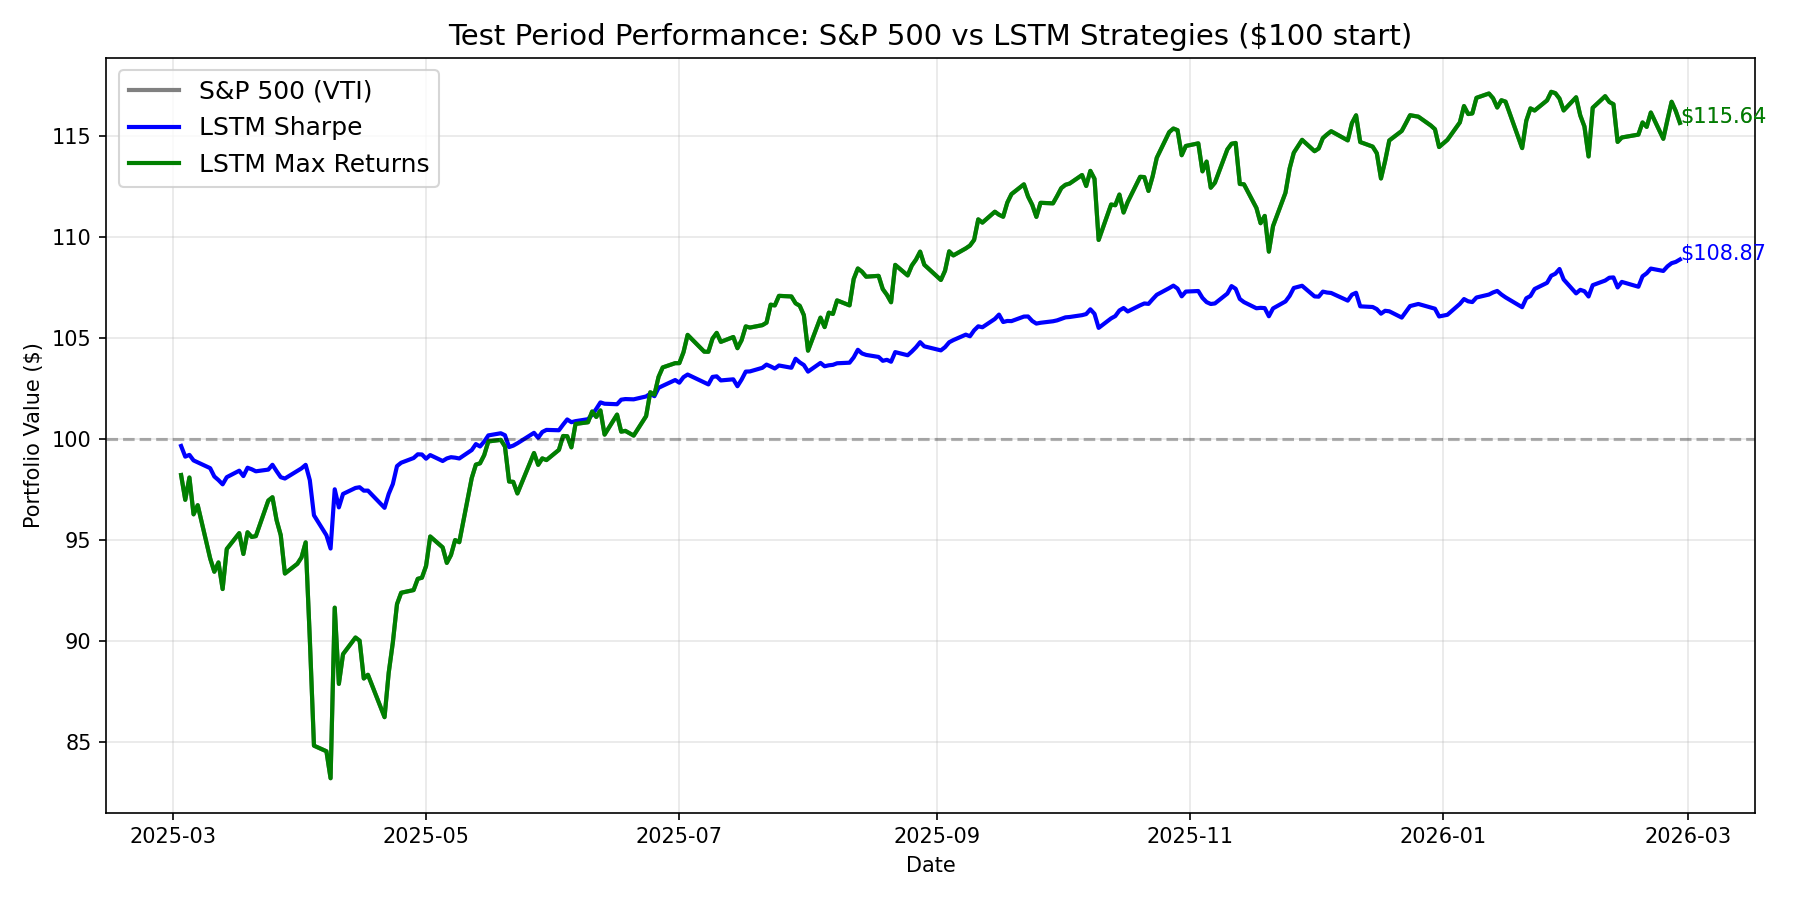
\includegraphics[width=0.85\textwidth]{test_performance.png}
\end{center}

\begin{columns}
\begin{column}{0.33\textwidth}
\centering
\textbf{S\&P 500}\\+15.64\%\\Max DD: $-$16\%
\end{column}
\begin{column}{0.33\textwidth}
\centering
\textbf{LSTM Sharpe}\\+8.87\%\\Max DD: $-$5\%
\end{column}
\begin{column}{0.33\textwidth}
\centering
\textbf{Key Insight}\\Lower return, but\\3$\times$ less drawdown
\end{column}
\end{columns}

\vspace{0.2cm}
\small During the April 2025 crash, S\&P dropped 16\% while our LSTM only dipped 5\%. \textbf{The model protects capital during uncertainty} --- critical for a scored competition.
\end{frame}

% ============================================================
\begin{frame}{Why This Matters for Scoring}

\textbf{Competition rubric: Performance \& Risk (40\%)}
\begin{quote}
``Teams that generate strong returns while \textit{avoiding large losses} receive higher scores.''
\end{quote}

\vspace{0.3cm}

\begin{table}
\centering
\begin{tabular}{lcc}
\toprule
& \textbf{S\&P 500 (buy \& hold)} & \textbf{Our LSTM} \\
\midrule
Return (test period) & +15.64\% & +8.87\% \\
Max Drawdown & $-$16\% & $-$5\% \\
Risk-adjusted (Sharpe) & Lower & \textbf{Higher} \\
\bottomrule
\end{tabular}
\end{table}

\vspace{0.3cm}

In a 2-week competition window with tariffs, geopolitical uncertainty, and elevated volatility, \textbf{capital preservation is as important as returns}.

\vspace{0.2cm}

The LSTM dynamically shifts toward defensive assets (bonds, commodities, volatility) when market conditions deteriorate.
\end{frame}

% ============================================================
\begin{frame}{Strategy 2: RSI-2 Mean Reversion on QQQ (5\%)}

\textbf{Concept:} Buy extreme dips in QQQ, sell the bounce. Historically 91\% win rate on large-cap ETFs.

\vspace{0.3cm}

\textbf{Rules:}
\begin{itemize}
    \item Compute 2-period RSI from daily closing prices:
    $$\text{RSI}(2) = 100 - \frac{100}{1 + \frac{\text{avg gain}}{\text{avg loss}}} \quad \text{(over last 2 days)}$$
    \item \textbf{Buy} when RSI(2) $< 10$ (QQQ had a sharp 1--2 day drop)
    \item \textbf{Sell} when RSI(2) $> 50$ (bounce happened, take profit)
    \item Long-only. Typical hold: 1--5 days.
\end{itemize}

\vspace{0.3cm}

\textbf{Why QQQ?} More volatile than SPY (tech-heavy), so RSI(2) triggers more often. In uncertain markets, sharp drops and bounces are frequent --- this strategy is designed to exploit that.

\vspace{0.2cm}

\textbf{Risk management:} Only 5\% allocation limits downside exposure.
\end{frame}

% ============================================================
\begin{frame}{Strategy 3: Price vs 10-day SMA on SPY (5\%)}

\textbf{Concept:} Simple momentum filter. Hold SPY when it's trending up, step aside when it breaks down.

\vspace{0.3cm}

\textbf{Rules:}
\begin{itemize}
    \item Compute 10-day Simple Moving Average of SPY closing prices:
    $$\text{SMA}(10) = \frac{1}{10}\sum_{i=1}^{10} \text{Close}_i$$
    \item \textbf{Buy} when current price $>$ 10-day SMA (short-term uptrend)
    \item \textbf{Sell} when current price $<$ 10-day SMA (trend broken)
    \item Long-only. Typical hold: 3--7 days.
\end{itemize}

\vspace{0.3cm}

\textbf{Complements RSI-2:}
\begin{itemize}
    \item RSI-2 buys \textit{fear} (sharp drops $\rightarrow$ bounce)
    \item SMA-10 rides \textit{momentum} (sustained uptrends)
    \item Different signals, different timing --- diversification
\end{itemize}
\end{frame}

% ============================================================
\begin{frame}{How the Three Strategies Work Together}

\begin{center}
\begin{tabular}{lccc}
\toprule
\textbf{Market Regime} & \textbf{LSTM (90\%)} & \textbf{RSI-2 (5\%)} & \textbf{SMA-10 (5\%)} \\
\midrule
Bull market & Heavy stocks (VTI) & Inactive (RSI high) & Holding SPY \\
Sharp crash & Shifts to bonds/vol & \textbf{Buys the dip} & Sells (protection) \\
Bounce/recovery & Rebalances back & \textbf{Sells for profit} & Buys back in \\
Sideways/choppy & Diversified allocation & Waits for signal & May whipsaw \\
\bottomrule
\end{tabular}
\end{center}

\vspace{0.5cm}

\begin{block}{Portfolio Construction Philosophy}
\begin{itemize}
    \item \textbf{90\% LSTM} --- AI-driven macro allocation across asset classes
    \item \textbf{5\% RSI-2} --- Tactical dip-buying for short-term alpha
    \item \textbf{5\% SMA-10} --- Trend-following overlay on SPY
\end{itemize}
Core + satellite approach: the LSTM is the core; RSI-2 and SMA-10 are tactical satellites.
\end{block}
\end{frame}

% ============================================================
\begin{frame}{Risk Management}

\textbf{Multiple layers of risk control:}

\vspace{0.3cm}

\begin{enumerate}
    \item \textbf{Asset diversification} --- LSTM allocates across stocks, bonds, commodities, and volatility. Not concentrated in a single asset.

    \item \textbf{Sharpe-optimized model} --- Trained to minimize drawdowns, not just maximize returns. Automatically shifts to defensive assets in downturns.

    \item \textbf{Position sizing} --- 90/5/5 split ensures no single strategy can significantly damage the portfolio.

    \item \textbf{Daily rebalancing} --- Adjusts positions every trading day at 3:50 PM ET. Doesn't hold stale positions.

    \item \textbf{Long-only} --- No short selling, no leverage, no options. Simple equity/ETF positions only.

    \item \textbf{Market orders before close} --- All orders execute during market hours at real-time prices. No overnight fill uncertainty.
\end{enumerate}
\end{frame}

% ============================================================
\begin{frame}{Execution \& Infrastructure}

\begin{columns}
\begin{column}{0.5\textwidth}
\textbf{Architecture:}
\begin{itemize}
    \item Linux server running 24/7
    \item 3 Python scripts as systemd services
    \item Auto-restart on failure
    \item All trades via Alpaca REST API
    \item Paper trading account (\$1M)
\end{itemize}

\vspace{0.3cm}

\textbf{Tech Stack:}
\begin{itemize}
    \item Python 3.12
    \item PyTorch (LSTM inference)
    \item alpaca-py SDK
    \item systemd for process management
\end{itemize}
\end{column}
\begin{column}{0.5\textwidth}
\textbf{Daily Schedule (all times ET):}

\vspace{0.2cm}

\begin{tabular}{cl}
\toprule
\textbf{Time} & \textbf{Action} \\
\midrule
3:45 PM & LSTM fetches data \\
3:45 PM & LSTM runs model \\
3:46 PM & LSTM submits orders \\
3:50 PM & RSI-2 checks signal \\
3:50 PM & SMA-10 checks signal \\
3:51 PM & All orders filled \\
4:00 PM & Market closes \\
\bottomrule
\end{tabular}

\vspace{0.3cm}

\textbf{Execution quality:}\\
Market orders with notional sizing.\\
No overtrading --- max 4--6 orders/day.\\
Efficient use of buying power.
\end{column}
\end{columns}
\end{frame}

% ============================================================
\begin{frame}{Addressing the Scoring Rubric}

\begin{table}
\centering
\begin{tabular}{p{3.5cm}cp{7cm}}
\toprule
\textbf{Criteria} & \textbf{Weight} & \textbf{Our Approach} \\
\midrule
Performance \& Risk & 40\% & Sharpe-optimized LSTM protects against drawdowns. Diversified across 4 asset classes + 2 tactical strategies. \\
\addlinespace
Execution Quality & 20\% & Daily rebalancing (not overtrading). Notional orders for precise sizing. All orders before close. Max 4--6 orders/day. \\
\addlinespace
Strategy Review & 40\% & Clear, explainable strategies with mathematical foundations. Backtested on 10 years of data. Robust risk management framework. \\
\bottomrule
\end{tabular}
\end{table}
\end{frame}

% ============================================================
\begin{frame}{Summary}

\begin{block}{Three strategies, one goal: risk-adjusted returns}
\begin{enumerate}
    \item \textbf{LSTM Portfolio (90\%)} --- AI allocates across stocks, bonds, commodities, and volatility daily. Trained to maximize Sharpe ratio. Protects capital in downturns.
    \item \textbf{RSI-2 on QQQ (5\%)} --- Buys extreme dips, sells bounces. 91\% historical win rate. Designed for volatile markets.
    \item \textbf{Price vs 10-SMA on SPY (5\%)} --- Rides short-term momentum, exits when trend breaks.
\end{enumerate}
\end{block}

\vspace{0.3cm}

\textbf{Why we believe this will perform well:}
\begin{itemize}
    \item Current market uncertainty (tariffs, geopolitics) favors defensive allocation
    \item LSTM dynamically shifts to safe havens when conditions deteriorate
    \item Competition scores \textit{risk-adjusted} performance, not just raw P\&L
    \item Fully autonomous --- no manual intervention needed for 2 weeks
\end{itemize}

\vspace{0.3cm}
\centering
\textbf{GitHub:} \texttt{github.com/verma-bipul/Algo-Trade-UMN-Team4}
\end{frame}

\end{document}
